\section{Алгоритмы решения задач с данными Коши. Примеры.}\label{sec:ch4/sec4}

%VYC0036
\subsection{
    Решение задачи сложного теплообмена
    с граничными условиями типа коши
}\label{subsec:ch4/sec4/subsec1}

Представим итерационный алгоритм решения задачи оптимального управления.
Пусть $\tilde J_\lambda(u)=J_\lambda(\theta(u), u)$, где $\theta(u)$ компонента решения
задачи~\eqref{eq:2_2:eq1},\eqref{eq:2_2:bc2}, соответствующая управлению $u\in U$.

В соответствии с~\eqref{eq:2_2:as} градиент функционала $\tilde J_\lambda(u)$ равен
\[
    \tilde J'_\lambda (u) = \lambda u - p_2.
\]
Здесь $p_2$ -- соответствующая компонента сопряженного
состояния из системы~\eqref{eq:2_2:as}, где $\hat{\theta}\coloneqq\theta(u)$.

%\begin{algorithm}[H]
%    \caption{Алгоритм градиентного спуска}
%    \label{alg:algorithm}
%    \begin{algorithmic}[1]
%        \State Выбираем значение градиентного шага $\varepsilon$,
%        \State Выбираем количество итераций $N$,
%        \State Выбираем начальное приближение для управления $u_0 \in U$,
%        \For{$k \gets 0,1,2,\dots,N$}
%            \State Для данного $u_k$ рассчитываем состояние $y_k = \{\theta_k, \varphi_k\}$ --
%            решение задачи~\eqref{eq:2_2:eq1},\eqref{eq:2_2:bc1}.
%            \State Рассчитываем значение функционала качества $J_\lambda(\theta_k, u_k)$.
%            \State Рассчитываем сопряженное состояние $p_k=\{p_{1k},p_{2k}\}$ из уравнений~\eqref{eq:2_2:oc1},
%            где $ \hat{\theta} \coloneqq \theta_k, \hat{u}=u_k$.
%            \State Пересчитываем управление $u_{k+1} = u_k - \varepsilon (\lambda u_k - p_2)$
%        \EndFor
%    \end{algorithmic}
%\end{algorithm}

Значение параметра $\varepsilon$ выбирается эмпирически таким образом, чтобы значение
$\varepsilon (\lambda u_k - p_2)$ являлось существенной поправкой для $u_{k+1}$.
Количество итераций $N$ выбирается достаточным для выполнения условия
$J_\lambda(\theta_k, u_k) - J_\lambda(\theta_{k+1}, u_{k+1}) < \delta$, где $\delta>0$
определяет точность расчетов.

Примеры, рассмотренные ниже, иллюстрируют работоспособность предложенного алгоритма при
малых, что важно, значениях параметра регуляризации $\lambda \leq 10^{-12}$.
В первом примере выполнены тестовые расчеты для куба.
Во втором примере приводится сравнение расчетов по
предложенному алгоритму с результатами работы~\cite{Chebotarev2019Problem}.

Отметим, что для численного решения прямой задачи с заданным управлением использовался
метод простой итерации для линеаризации задачи и ее решения методом конечных элементов.
Решение сопряженной системы, которая является линейной при заданной температуре, не вызывает трудностей.
Для численного моделирования использовался солвер FEniCS~\cite{fenics, dolfin}.

Исходный код экспериментов можно найти по ссылке~\cite{mesenev-github}.

\textbf{Пример 1.}

Приведем примеры расчетов для куба $\Omega = {(x, y, z), 0 \leq x,y,z \leq l}$.
Будем считать, что $l=1~\text{см}$, $a = 0.006[\text{см}^2/\text{c}]$,
$b=0.025[\text{см}/\text{с}]$, $\kappa_a=1[\text{см}^{-1}]$, $\alpha = 0.(3)[\text{см}]$.
Указанные параметры соответствуют стеклу~\cite{Grenkin2016a}.
Параметр регуляризации $\lambda=10^{-12}.$

Пусть граничные данные $r$ и $u$ в~\eqref{eq:2_2:bc1} имеют вид:
\begin{gather*}
    r = 0.7,\\
    u = \hat u = 0.5.
\end{gather*}
Далее рассчитываем состояние $\theta$ и $\varphi$ как решение
задачи~\eqref{eq:2_2:eq1},\eqref{eq:2_2:bc1} и в качестве $\theta_b$
выбираем граничное значение функции $\theta$ на $\Gamma$.
Значения нормальной производной $\partial_n\theta$ на $\Gamma$
должны соответствовать значениям $q_b=r/a-\theta_b$.
Применяя предложенный алгоритм с начальным приближением $u_0 = 0.1$,
находим приближенное решение $\{\theta_\lambda, \varphi_\lambda, u_\lambda\}$ задачи (CP).
Для демонстрации того, что алгоритм находит приближенное решение задачи с данными
Коши для температуры, важно сравнить значения $\partial_n\theta_\lambda$ на $\Gamma$ с $q_b.$

На рисунке~\ref{fig:img_test_1_iso} представлен модуль относительного
отклонения $\partial_n\theta_\lambda$ от $q_b$ на грани куба в плоскости $z=l$,
где $\partial_n\theta_\lambda=\partial\theta_\lambda/\partial z$,
а также динамика функционала качества, определяющего норму
разности $\|\theta_\lambda -\theta_b\|^2_\Gamma$ на рисунке~\ref{fig:quality_1}.
На остальных гранях куба значения относительного
отклонения имеют тот же порядок малости.

\begin{figure}[h!]
    \centering
    \subfloat[$|\partial_n\theta_\lambda-q_b|/|q_b|$]
    {\label{fig:img_test_1_iso} 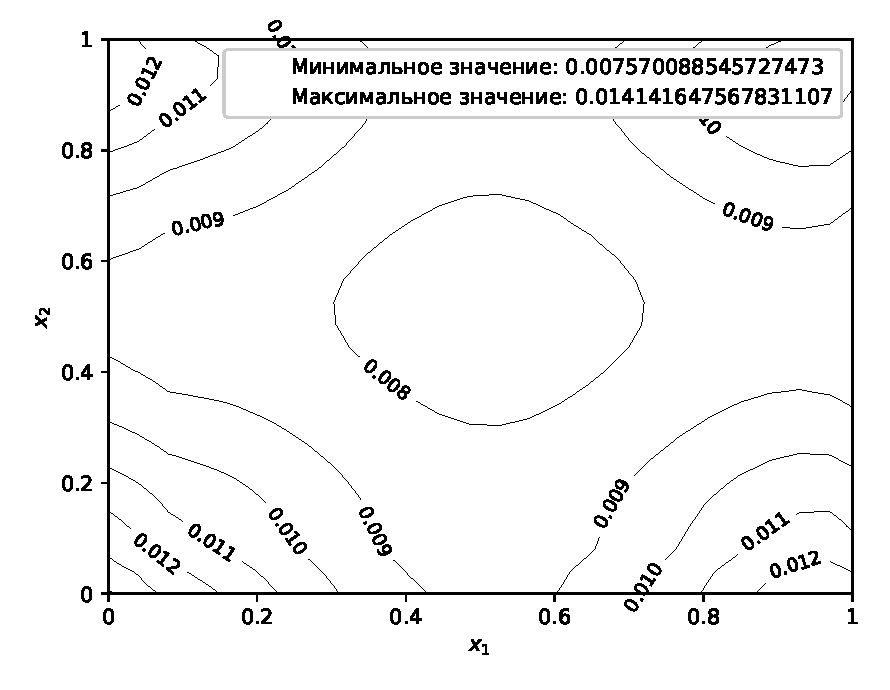
\includegraphics[width=.49\linewidth]{jvm-2020/exp1/theta_n_diff_iso}}
    \subfloat[Изменение функционала качества по итерациям]
    {\label{fig:quality_1} \includegraphics[width=.49\linewidth]{jvm-2020/exp1/quality}}
    \caption{Результаты первого эксперимента}
\end{figure}

\textbf{Пример 2.}
Сравним работу предложенного алгоритма с результатами статьи~\cite{Chebotarev2019Problem},
где соавтором был один из авторов данной работы.
Задача рассматривается в области $\Omega \times (-L,L)$,
где $\Omega = \{ x = (x_1,x_2) \colon 0 < x_{1,2} < d\}$
и при больших $L$ сводится к двумерной задаче с вычислительной областью $\Omega$.
Выбраны следующие значения параметров задачи:
$d = \mathrm{1(m)}$, $a = 0.92~10^{-4}~\mathrm{(m^2/s)}$, $b= 0.19~\mathrm{(m/s)}$,
$\alpha = 0.0333~\mathrm{(m)}$ и $\kappa_a = 1~\mathrm{(m^{-1})}$.
Параметры соответствуют воздуху при нормальном атмосферном давлении и температуре 400$^\circ$C\@.

Функции $\theta_b$, $q_b$ в краевом условии~\eqref{eq:2_2:bc2} заданы следующим образом:
$\theta_b = \widehat{\theta}|_{\Gamma}$, $q_b = \partial_n \widehat{\theta}|_{\Gamma}$, где
$\widehat{\theta} = (x_1-0.5)^2 - 0.5x_2+0.75$.

Приближенное решение задачи с данными Коши, представленное в~\cite{Chebotarev2019Problem}
получено путем решения эллиптической задачи четвертого
порядка для температуры методом установления по времени.
Использовались $H^2$ конформные конечные элементы Богнера-Фокса-Шмитта и
солвер FeliCs, разработанный в техническом университете Мюнхена.
Решение стабилизировалось через 120 секунд, но вычисления на каждом временном
шаге потребовали довольно значительных затрат~\cite{Chebotarev2019Problem}.

На рис.~\ref{fig:theta_auto_2} представлено температурное поле, полученное
предложенным в данной статье методом, достаточно
точно совпадающее с результатом в~\cite{Chebotarev2019Problem}.
Величина $\|\partial_n\theta_\lambda-q_b\|_{L^2(\Gamma)}/\|q_b\|_{L^2(\Gamma)}$ равна $~0.000567$.
Значение функционала качества, определяющего норму разности $\|\theta_\lambda -\theta_b\|^2_\Gamma$,
равно $~0.000255$ и стабилизируется после 10 итераций~\ref{fig:quality_2}.

\begin{figure}[h!]
    \centering
    \subfloat[Полученное решение $\theta$]
        { \label{fig:theta_auto_2} 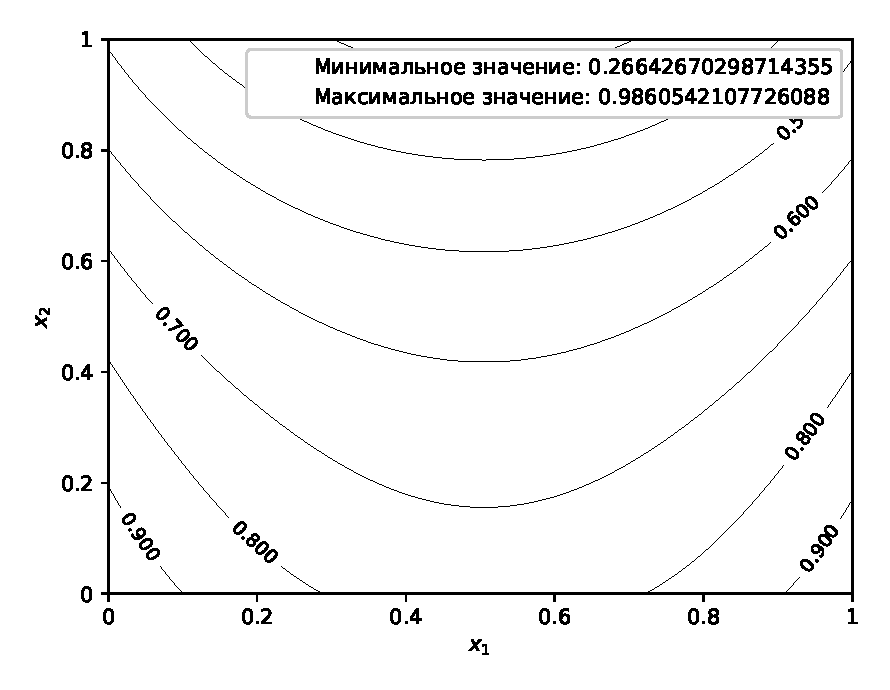
\includegraphics[width=.49\linewidth]{jvm-2020/exp2/theta_auto} }
    \subfloat[Изменение функционала качества]
    { \label{fig:quality_2} \includegraphics[width=.49\linewidth]{jvm-2020/exp2/quality} }
    \caption{Результаты второго эксперимента}
\end{figure}

Представленные численные примеры иллюстрируют, что предложенный алгоритм успешно справляется
с нахождением численного решения задачи~\eqref{eq:2_2:eq1}--\eqref{eq:2_2:bc2}.


\textbf{Пример 3.}
Положим в условии~\eqref{eq:2_2:bc1}
$r=0.8 \cos (x)+0.1,\; u=\hat{u}=y$.
Далее рассчитываем состояние $\theta$ и $\varphi$ как решение
задачи~\eqref{eq:2_2:eq1}--\eqref{eq:2_2:bc2}
и в качестве $\theta_{b}$ выбираем граничные значения функции $\theta$ на Г.
Применяя предложенный алгоритм с начальным приближением $u_{0}=0.1$,
находим приближенное решение задачи $(C)$.
Квадрат разницы тестового и найденного решения представлен на рисунке~\ref{fig:4_4:dvmg-1a},
а также динамика функционала качества рисунке~\ref{fig:4_4:dvmg-1b}.
\begin{figure}[h!]
    \centering
    \subfloat[$\left(\hat{u}-u_{100}\right)^{2}$]
    { \label{fig:4_4:dvmg-1a} 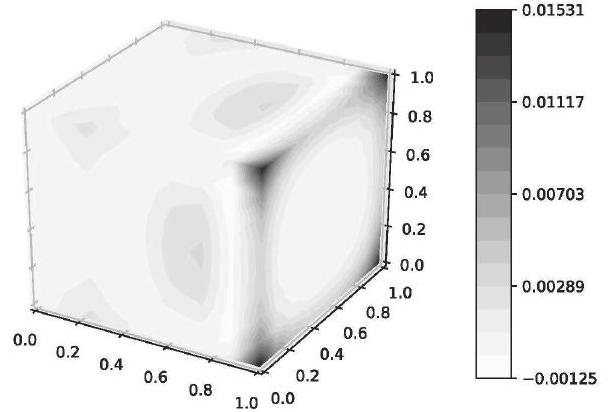
\includegraphics[width=.49\textwidth]{jvm-2020/dvmg/1a} }
    \subfloat[Изменение функционала в зависимости от числа итераций]
    { \label{fig:4_4:dvmg-1b} 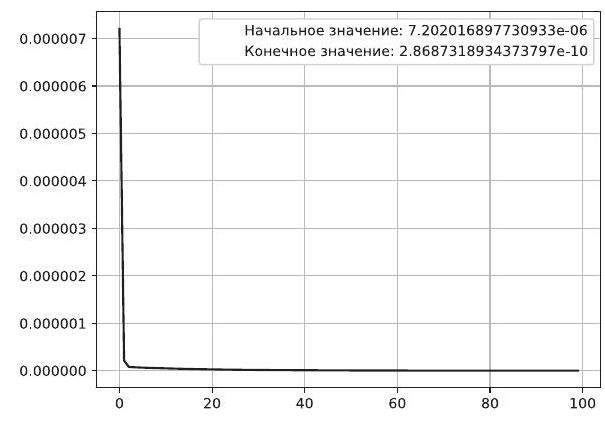
\includegraphics[width=.49\linewidth]{jvm-2020/dvmg/1b} }
    \caption{Результаты третьего эксперимента}
\end{figure}


\textbf{Пример 4.}
Зададим функции $\theta_{b}, q_{b}$ в краевом условии~\eqref{eq:2_2:bc2}
следующим образом:

\[
    \theta_{b}=0.1 z+0.3, \quad q_{b}=
    \begin{cases}
        0.11, & \text { если } z=1, \\
        0, & \text { если } 0<z<1, \\
        -0.15, & \text { если } z=0.
    \end{cases}
\]


В данном примере оптимальное управление $u$ в качестве тестового не задается.
На рисунках~\ref{fig:4_4:dvmg-2a}~\ref{fig:4_4:dvmg-2b} представлен результат работы алгоритма.
\begin{figure}[h!]
    \centering
    \subfloat[Оптимальное управление]
    { \label{fig:4_4:dvmg-2a} 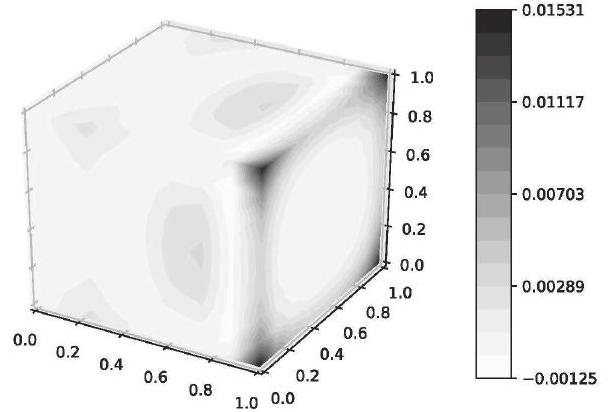
\includegraphics[width=.49\textwidth]{jvm-2020/dvmg/1a} }
    \subfloat[Изменение функционала в зависимости от числа итераций]
    { \label{fig:4_4:dvmg-2b} 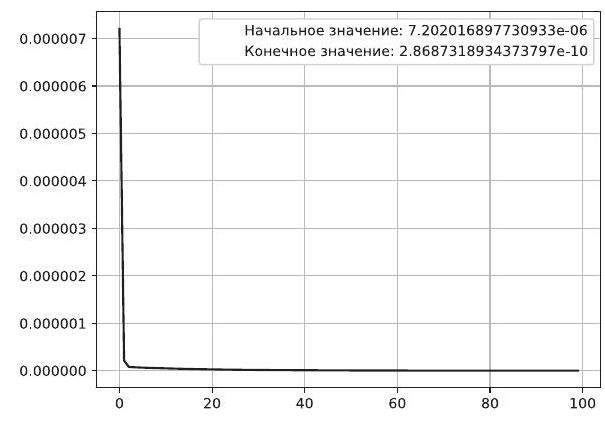
\includegraphics[width=.49\linewidth]{jvm-2020/dvmg/1b} }
\end{figure}


Компоненты состояния, соответствующие найденному управлению, представлены на
рисунках~\ref{fig:4_4:dvmg-3a}\ref{fig:4_4:dvmg-3b}.

\begin{figure}[h!]
    \centering
    \subfloat[Температура $\theta$]
        { \label{fig:4_4:dvmg-3a} 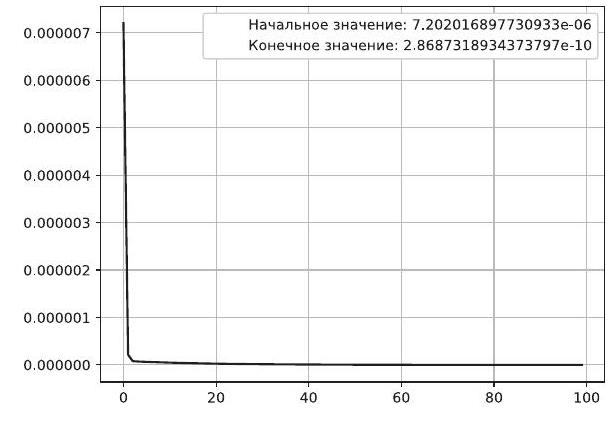
\includegraphics[width=.49\textwidth]{jvm-2020/dvmg/3a} }
    \subfloat[Излучение $\varphi$]
        { \label{fig:4_4:dvmg-3b} 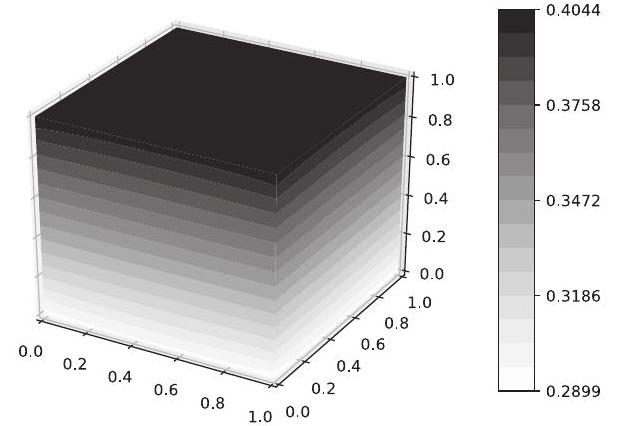
\includegraphics[width=.49\linewidth]{jvm-2020/dvmg/3b} }
\end{figure}

\subsection{
    Задача сложного теплообмена с условиями
    Коши для температуры на части границы
}\label{subsec:ch4/sec4/subsec2}
    %jvm-mesenev-chebotarev

Представим итерационный алгоритм решения задачи оптимального управления.
Пусть $\tilde J_\lambda(u)=J_\lambda(\theta(u), u)$,
где $\theta(u)$ компонента решения
задачи~\eqref{eq:2_4:eq1},\eqref{eq:2_4:bc2},
соответствующая управлению $u\in U$.

В соответствии с~\eqref{eq:2_4:as} градиент функционала $\tilde J_\lambda(u)$ равен
\[ \tilde J'_\lambda (u) = \lambda u - p_2. \]
Здесь $p_2$ -- соответствующая компонента сопряженного состояния из системы ~\eqref{eq:2_4:as},
где $\hat{\theta}\coloneqq\theta(u)$.

%    \begin{algorithm}[H]
%        \caption{Алгоритм градиентного спуска}
%        \label{alg:algorithm}
%        \begin{algorithmic}[1]
%            \State Выбираем значение градиентного шага $\varepsilon$,
%            \State Выбираем количество итераций $N$,
%            \State Выбираем начальное приближение для управления $u_0 \in U$,
%            \For{$k \gets 0,1,2,\dots,N$}
%                \State Для данного $u_k$ рассчитываем состояние $y_k = \{\theta_k, \varphi_k\}$ --
%                решение задачи~\eqref{eq1},\eqref{bc1}.
%                \State Рассчитываем значение целевого функционала $J_\lambda(\theta_k, u_k)$.
%                \State Рассчитываем сопряженное состояние $p_k=\{p_{1k},p_{2k}\}$ из уравнений ~\eqref{OC1},
%                где $ \hat{\theta} \coloneqq \theta_k, \hat{u}=u_k$.
%                \State Пересчитываем управление $u_{k+1} = u_k - \varepsilon (\lambda u_k - p_2)$
%            \EndFor
%        \end{algorithmic}
%    \end{algorithm}
Значение параметра $\varepsilon$ выбирается эмпирически таким образом, чтобы значение
$\varepsilon (\lambda u_k - p_2)$ являлось существенной поправкой для $u_{k+1}$.
Количество итераций $N$ выбирается достаточным для выполнения условия
$J_\lambda(\theta_k, u_k) - J_\lambda(\theta_{k+1}, u_{k+1}) < \delta$, где $\delta > 0$
определяет точность расчетов.

Примеры, рассмотренные ниже, иллюстрируют работоспособность предложенного алгоритма при
малых, что важно, значениях параметра регуляризации $\lambda \leq 10^{-12}$.
В первом примере выполнены тестовые расчеты для куба.
Во втором примере рассмотрен куб с внутренней полостью.
Для численного решения прямой задачи с заданным управлением использовался
метод Ньютона для линеаризации задачи и ее решения методом конечных элементов.
Решение сопряженной системы, которая является линейной при заданной температуре, не вызывает трудностей.
Для численного моделирования использовался солвер FEniCS~\cite{fenics},\cite{dolfin}.

Исходный код экспериментов можно найти по ссылке~\cite{mesenev-github}.

\textbf{Пример 1.}
Рассмотрим куб $\Omega = {(x, y, z), 0 \leq x,y,z \leq l}$ с границей
$\Gamma \equiv \Gamma_1 \cup \Gamma_2$, где
\[
    \Gamma_1 = \{(x, y, z), 0 \leq x,y, \leq l, z \in 0, l\}, \;
    \Gamma_2 = \partial \Omega \setminus \hat{\Gamma_1}.
\]
Будем считать, что
$l = 1~\text{см}$,
$a = 0.6[\text{см}^2/\text{c}]$,
$b = 0.025[\text{см}/\text{с}]$,
$\kappa_a = 1[\text{см}^{-1}]$,
$\alpha = 0.(3)[\text{см}]$.
Указанные параметры соответствуют стеклу~\cite{Grenkin2016a}.
Параметр регуляризации $\lambda=10^{-12}$.

Пусть граничные данные $q_b$ и $\theta_b$ в~\eqref{eq:2_4:bc1},\eqref{eq:2_4:bc2} имеют вид:
\begin{gather*}
    q_b = 0.5, \quad
    \theta_b = 0.1 + z/2
\end{gather*}
на все границе, а также начальное управление $u_0 = 0$.
Используя предложенный алгоритм решим задачу оптимального управления.

\begin{figure}[h!]
    \centering
    \subfloat[$\theta|_{z=1} $]
    {
        \label{fig:1_theta}
        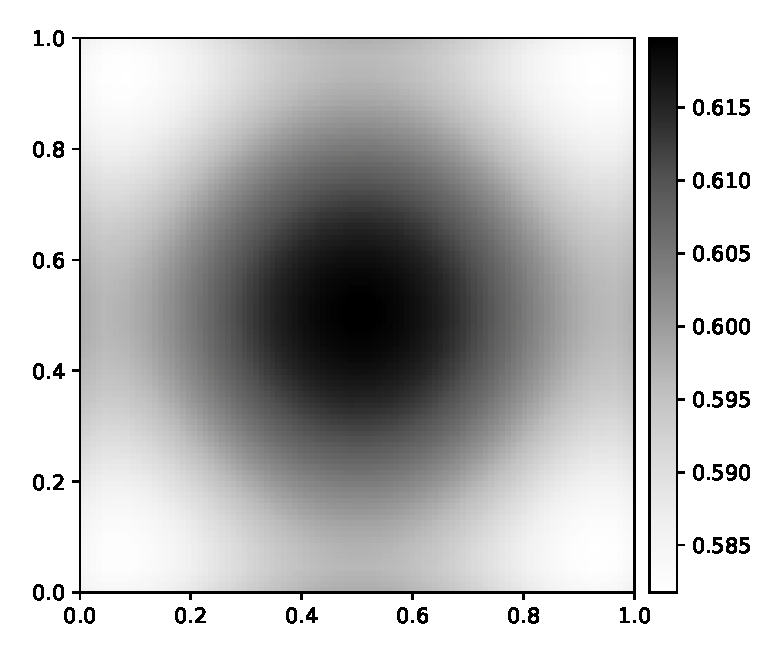
\includegraphics[width=.4\linewidth]{jvm-2022/1_theta}
    }
    \subfloat[$\phi|_{z=1} $]
    {
        \label{fig:1_phi}
        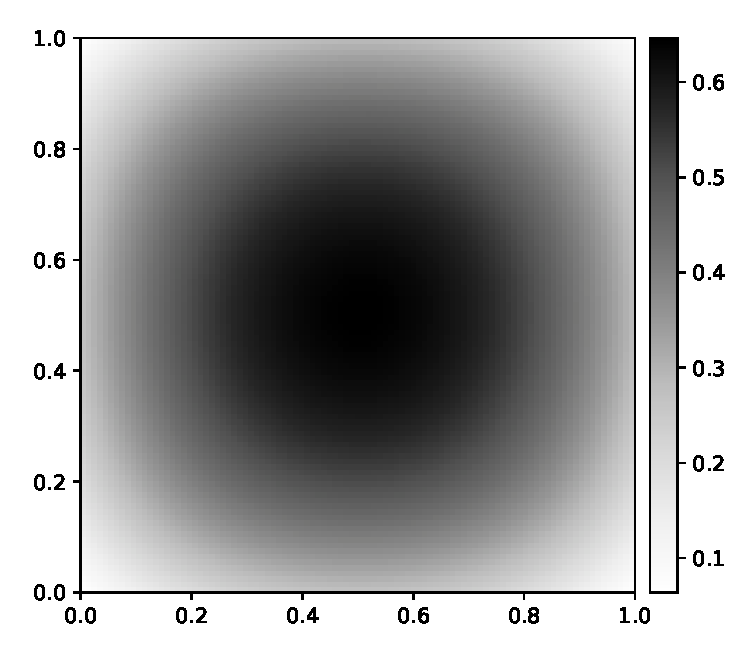
\includegraphics[width=.4\linewidth]{jvm-2022/1_phi}
    }
    \caption{Результаты первого эксперимента}
    \label{fig:4_4:1}
\end{figure}

На фиг.~\ref{fig:1_theta},~\ref{fig:1_phi} представлены
полученные решения $\theta$ и $\phi$.
Начальное значение функционала качества равно $~0.025$ и
через сотню итераций становится равным $~5.e-05$.

\textbf{Пример 2.}
Рассмотрим двумерный случай: имеется квадрат
$S = \{(x, y), 0 \leq x,y,z \leq 1~\text{см.}\}$ с
круговой полостью $R$ с центром $b_0 =\{0.5, 0.5\}$
$R = \{r, \| r - b_0 \| \leq 0.15~\text{см.} \}$.
Рассматриваемая область $\Omega = S \setminus R$.
$\Gamma \equiv \partial \Omega = \partial C \cup \partial B$ при чём
\[
    \Gamma_2 = \partial R,
    \Gamma_1 = \partial S \setminus \Gamma_2.
\]
Параметры среды возьмём из примера 1.
Граничные данные $q_b$ и $\theta_b$ положим равными
\begin{gather*}
    \theta_b = 0.5, \\
    q_b =
    \begin{cases}
        0.2, & \text{если } x \in \Gamma_1 \\
        -0.2, & \text{если } x \in \Gamma_2.
    \end{cases}
\end{gather*}
\begin{figure}[h!]
    \centering
    \subfloat[$\theta$]
    {
        \label{fig:2_theta}
        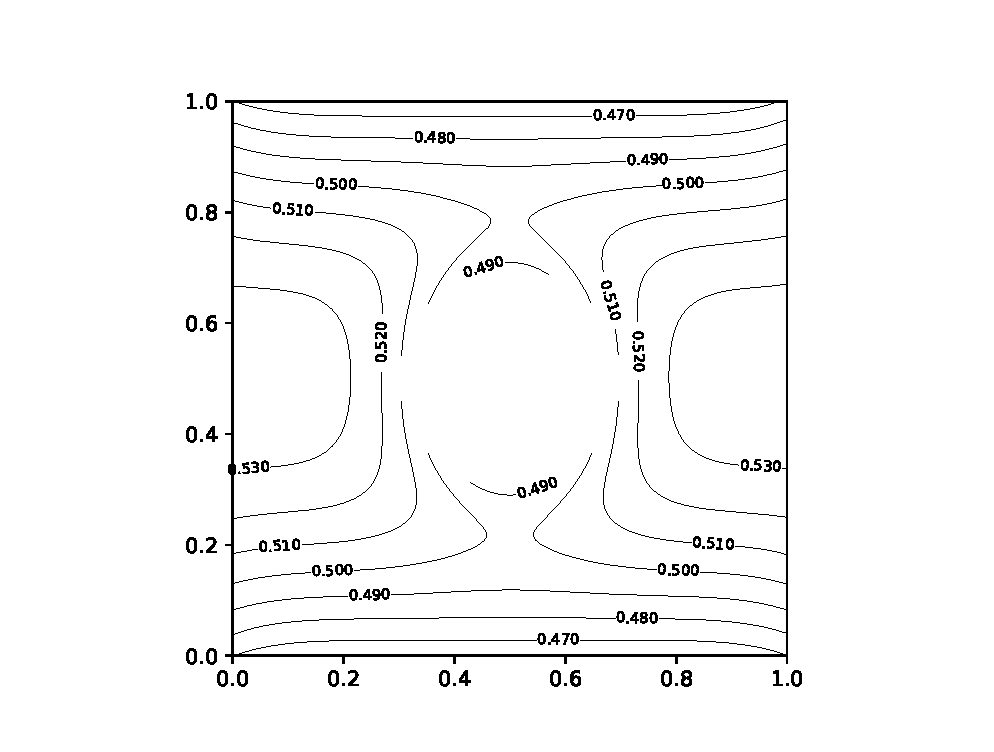
\includegraphics[width=.5\linewidth]{jvm-2022/2_theta}
    }
    \subfloat[$\phi$]
    {
        \label{fig:2_phi}
        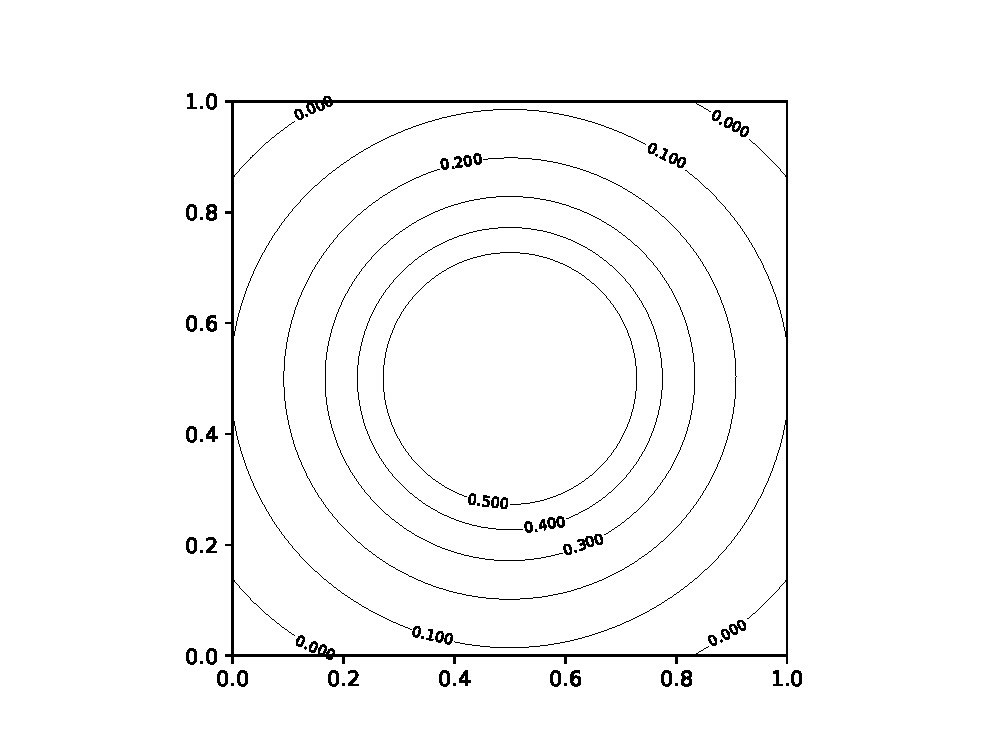
\includegraphics[width=.5\linewidth]{jvm-2022/2_phi}
    }
    \caption{Результаты второго эксперимента}
    \label{fig:2}
\end{figure}
Начальное значение функционала качества $~0.045$.
После тридцати итераций $~6.2-05$.
Полученное состояние представлено рисунками ~\ref{fig:2_theta},\ref{fig:2_phi}.


Представленные численные примеры демонстрируют,
что предложенный алгоритм успешно справляется
с нахождением численного решения задачи~\eqref{eq:2_4:eq1}--\eqref{eq:2_4:bc2}.

